\documentclass[12pt]{article}
\usepackage[spanish]{babel}
\usepackage{amsmath}
\usepackage{graphicx}
\usepackage[utf8]{inputenc}
\usepackage{float} 
\title{\LaTeX}
\date{}
% Este es un comentario, no será mostrado en el documento final.
\begin{document}

\subsection{Ejercicio 2}
La idea de este ejercicio es hacer seis gaussianas bivariadas a partir de seis medias, calculadas por el estimador de máxima verosimilitud, y un sigma elegido a partir de la consigna. \newline
Para hacer esto primero transformo la imagen phantom en una matriz de ALTOxANCHOx3 (RGB) con el comando $imread$. Luego sumo todas las posiciones X e Y de un color, y las divido por la cantidad de pixeles que son de dicho color. De esta forma queda un vector de longitud dos (mu) conformado por la suma de todas las posiciones X dividido la cantidad de pixeles de ese color, y lo mismo para Y.\newline 
Para clasificar la imagen, recorro pixel por pixel toda la imagen y calculo el valor de las seis gaussianas en esa posición. Luego para escoger el color en un pixel, elijo el que me haya dado la probabilidad mas alta. 
\subsubsection{Resultados e Imágenes}
\begin{figure}[H]
\centering
\includegraphics[width=150mm]{tp1/phantom.png}
\caption{Imágen phantom real (verdad terrestre)}
\end{figure}
\begin{figure}[H]
\centering
\includegraphics[width=140mm]{tp1/1.jpg}
\caption{Imágen sintética con matrices de covarianza isotrópicas e iguales entre sí}
\includegraphics[width=140mm]{tp1/2.jpg}
\caption{Imágen sintética con matrices de covarianza diagonales y diferentes para cada clase}
\end{figure}
\begin{figure}[H]
\centering
\includegraphics[width=150mm]{tp1/3.jpg}
\caption{Imagen sintética con matrices de covarianza diferentes no-diagonales y diferentes}
 \label{fig:3}
\end{figure}
Para crear las matrices de confusión, creo dos matrices de dos dimensiones ALTOxANCHO (tamaño de la imagen phantom). \newline
\newline
\textbf{Predicciones:}\newline
En la primer matriz recorro pixel por pixel (a la hora de clasificar) colocando números del 1 al 6 en cada posición de esta nueva matriz indicando a que clase pertenece cada pixel (de acuerdo a la clase que haya dado la probabilidad mas alta).\newline\newline
\textbf{Verdad terrestre:}\newline
En la segunda matriz también recorro pixel por pixel y coloco los valores 1,2,3,4,5,6 para indicar a que clase pertenece, y el número 7 para los valores que no pertenecen a ninguna clase de la imagen phantom (no clasificados), ya que en algunas partes de la imagen se pixela y no se puede determinar cuál es la verdadera clase a la que pertenece dicho pixel. \newline
Luego para crear la matriz de confusión uso el comando $confusionmat$ ingresándole dos vectores (primer y segunda matriz apiladas en dos vectores) y un orden (1,2,3,4,5,6,7) con las clases. Las matrices de confusión se muestran al finalizar la compilación de cada archivo del ejercicio 2.\newline\newline
\textbf{Conclusión:}\newline
Se puede observar que, si consideramos la matriz de covarianza igual para cada clase, la separación entre las clases es muy cuadrada. En cambio, se redondea cuando ponemos matrices de covarianza distintas para cada clase. Las imágenes sintéticas no son perfectas, pero se asemejan muy bien a la original en cuanto a posición. \newline
Otro dato interesante es que para que la imagen sintética se acerque a la imagen original phantom se tiene que considerar una matriz de covarianza con valores grandes, ya que, si consideramos valores pequeños, la clasificación es muy estricta y la imagen generada será muy alejada a la original.
\subsection{Ejercicio 3}
En este ejercicio, genero tres Gaussianas trivariadas a partir del estimador de máxima verosimilitud de la media y el sigma (matriz de covarianza). Luego recorro, pixel por pixel, toda la imagen, y calculo la probabilidad de pertenecer a cada clase, con las tres Gaussianas.\newline
Primero transformo la imagen en una matriz de ANCHOxALTOX3 (RGB) con el comando $imread$.\newline 
Para generar las matrices de covarianza, utilizo una función auxiliar $matriz_cov$ que me devuelve el estimador de máxima verosimilitud del sigma, es decir, una matriz cuadrada de 3 dimensiones.\newline\newline 
Para generar las medias (mu) creo un vector de 3 posiciones. En cada posición, primero calculo la suma de todos los elementos de las submatrices ALTOxANCHOx1, ALTOxANCHOx2, ALTOxANCHOx3 (R, G y B) respectivamente. Luego las divido por la cantidad de elementos, y me queda un vector de longitud 3, es decir, el estimador de máxima verosimilitud de la media.\newline\newline
Por ultimo recorro, pixel por pixel, toda la imagen y calculo las probabilidades de que cada pixel pertenezca a cada una de las tres clases, y me quedo con la probabilidad mas alta. Luego lo pinto del color de dicha clase.\newline
 \begin{figure}[H]
\centering
\includegraphics[width=70mm]{tp1/circular.jpg}
\caption{Imágen real}
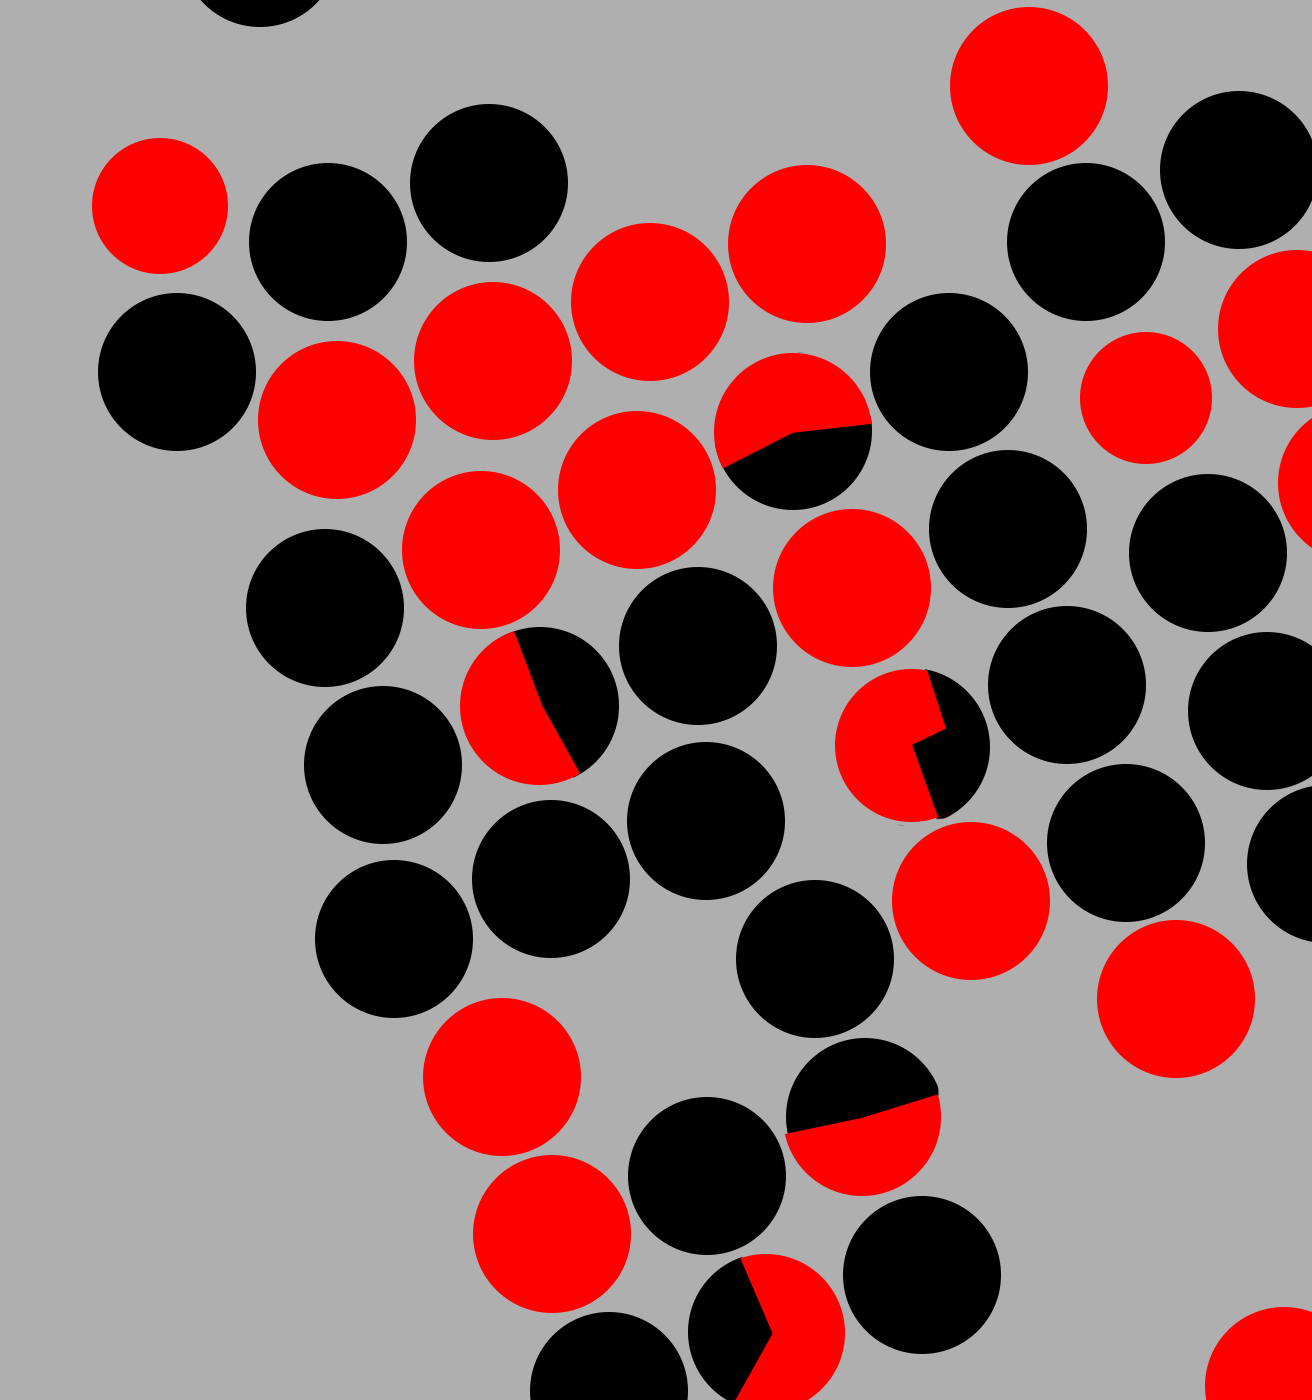
\includegraphics[width=70mm]{tp1/circular_verdad.png}
\caption{Imágen cultivo verdad terrestre}
\end{figure}
\begin{figure}[H]
\centering
\includegraphics[width=100mm]{tp1/circular_clasificada.png}
\caption{Imágen según clasificación}
\end{figure}
Para hacer la matriz de confusión, con un editor de imágenes creamos una imagen que ofrece la verdad terrestre, es decir, los datos clasificados de manera correcta.\newline 
Para crear la matriz de confusión, creo dos matrices de dos dimensiones ALTOxANCHO (tamaño de la imagen del cultivo).\newline\newline 
\textbf{Predicciones:}\newline
En la primer matriz recorro pixel por pixel (a la hora de clasificar) colocando números del 1 al 3 en cada posición de esta nueva matriz indicando a que clase pertenece cada pixel (de acuerdo a la clase que haya dado la probabilidad mas alta).\newline\newline
\textbf{Verdad terrestre:}\newline
En la segunda matriz también recorro pixel por pixel y coloco los valores 1,2,3 para indicar a que clase pertenece realmente. Luego para crear la matriz de confusión uso el comando confusionmat ingresándole dos vectores (primer y segunda matriz apiladas en dos vectores) y un orden (1,2,3) con las clases. La matriz de confusión se muestra al finalizar la compilación del ejercicio 3.\newline\newline
\textbf{Conclusión:}\newline
Lo interesante de este ejercicio es que la clasificación depende mucho de la selección de las regiones de entrenamiento, ya que a partir de estas se estima la media (Estimador de máxima verosimilitud) y las matrices de covarianza. Si se elige una región de entrenamiento demasiado grande, la clasificación va a ser muy laxa.\newline
Si se elige una región de entrenamiento muy pequeña, la clasificación va a ser muy estricta. Además, influye mucho que sección de la imagen seleccionamos como región de entrenamiento ya que, si tomamos regiones muy similares, se hace muy difícil decidir a qué clase pertenece cada pixel. 

\end{document}